\songchapter{Z}  % This is Chapter Z for singers/bands whose names start with "Z"

%%%%%%%%%%%%%%%%%%%%%%%%%%%%%
\songsection{周云蓬}	\index{Z!zhouyunpeng} % \songsection{}  This is the name of singer/band

%%%%%%%%%%%%%%%%%%%
\subsection{沉默如谜的呼吸} % This is the name of the album

\begin{figure}[htp] % Typically we provide the cover of the album
	\begin{center}
	  
\includegraphics[scale = 0.80]{z/zhouyunpeng/chenmorumi} % scale: size of the figure; {z/zhouyunpeng/chenmorumi}: name of the figure
% 	  \caption[labelInTOC]{沉默如谜的呼吸}
	  \label{fig:chenmorumi}
	\end{center}
\end{figure}

\begin{songs}{} % the song
  \beginsong{我听到某人在唱一首忧伤的歌}[by={词作:巫昂}, index={我听到某人在唱一首忧伤的歌}] % the song
	我们离开那间租来的房子	\\  % newline by "\\"
	悄悄都把灯拉灭	\\
	只剩下某人自己在屋中坐着	\\
	天已黑了	\\
	我听到他在唱一首忧伤的歌	\\
	\vspace{2ex}    % insert a vertical space
	这是夏天最后的一个黄昏	\\
	河里的水都越来越凉了	\\
	河边的水草忙着结婚生子	\\
	一片凄凉中	\\
	生活着一个热闹的家庭	\\
	而我们的家已经荡然无存	\\
	我们的家和稻谷捆扎在一起	\\
	在田野深处静静生长静静生长	\\
  \endsong
  
  \beginsong{}[by = {词作: }, index = {}] % another song
  
  \endsong
\end{songs}

%%%%%%%%%%%%%%%%%%%
\subsection{中国孩子}   % another album

\begin{figure}[htp]
	\begin{center}
	  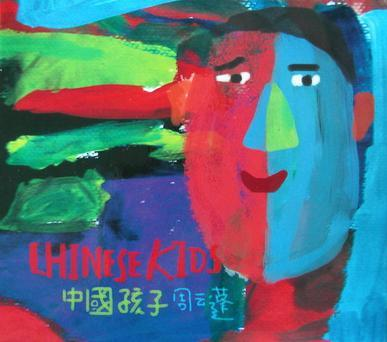
\includegraphics[scale = 0.50]{z/zhouyunpeng/zhongguohaizi}
% 	  \caption[labelInTOC]{中国孩子}
	  \label{fig:zhongguohaizi}
	\end{center}
\end{figure}

\begin{songs}{}
  \beginsong{悬棺}[index={悬棺}]
	一 二 三 四	\\
	悬在云间	\\
	上看不到你的天	\\
	下见不到我的地	\\
	秋天不用收粮食	\\
	冬天不必盖房子	\\
	\vspace{2ex}
	悬棺 悬棺在云间	\\
	上看不到你的天	\\
	下见不到我的地	\\
	秋天不用收粮食	\\
	冬天不必盖房子	\\
	\vspace{2ex}
	我们就住在云彩上面的棉花里	\\
	我们在棉花里偷偷地喝酒	\\
	踉踉跄跄一脚高山	\\
	踉踉跄跄一脚平原	\\
	踉踉跄跄一脚海洋	\\
	踉踉跄跄一脚沙滩	\\
	我们的身体是一只水桶	\\
	升上去空空荡荡	\\
	落下来装满了水	\\
	升上去空空荡荡	\\
	落下来装满了水	\\
	\vspace{2ex}
	悬在云间	\\
	上看不到你的天	\\
	下见不到我的地	\\
	秋天不用收粮食	\\
	冬天不必盖房子	\\
	\vspace{2ex}
	悬棺 悬棺在云间	\\
	上看不到你的天	\\
	下见不到我的地	\\
	秋天不用收粮食	\\
	冬天不必盖房子	\\
  \endsong
\end{songs}
%%%%%%%%%%%%%%%%%%%
\subsection{牛羊下山}

\begin{figure}[htp]
	\begin{center}
	  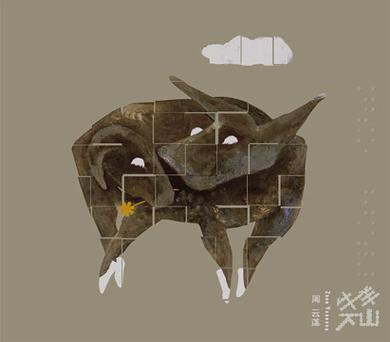
\includegraphics[scale = 0.50]{z/zhouyunpeng/niuyangxiashan}
% 	  \caption[labelInTOC]{牛羊下山}
	  \label{fig:niuyangxiashan}
	\end{center}
\end{figure}

\begin{songs}{}
  \beginsong{不会说话的爱情}[index={不会说话的爱情}]
	绣花绣的累了吗 \hspace{5mm} 牛羊也下山喽	\\
	我们烧自己的房子和身体 \hspace{5mm} 生起火来	\\
	解开你的红肚带 \hspace{5mm} 洒一床雪花白	\\
	普天下所有的水 \hspace{5mm} 都在你眼中荡开	\\
	没有窗亮着灯 \hspace{5mm} 没有人在途中	\\
	我们的木床唱起歌儿 \hspace{5mm} 说幸福它走了	\\
	我最亲爱的妹呀 \hspace{5mm} 我最亲爱的姐呀	\\
	我最可怜的皇后 \hspace{5mm} 我屋旁的小白菜	\\
	
	日子快到头了 \hspace{5mm} 果子也熟透了	\\
	我们最后一次收割对方 \hspace{5mm} 从此仇深似海	\\
	你去你的未来 \hspace{5mm} 我去我的未来	\\ 	
	我们只能在彼此的梦境里 \hspace{5mm} 虚幻得徘徊	\\
	徘徊在你的未来 \hspace{5mm} 徘徊在我的未来	\\
	徘徊在水里火里汤里 \hspace{5mm} 冒着热气期待	\\
	期待更美的人到来 \hspace{5mm} 期待更好的人到来	\\
	期待我们的灵魂附体 \hspace{5mm} 重新回来	\\
	重新回来 \hspace{5mm} 重新回来	\\
  \endsong
\end{songs}
%%%%%%%%%%%%%%%%%%%%%%%%%%%%%
\songsection{郑智化}	\index{Z!zhengzhihua} % another singer/band

%%%%%%%%%%%%%%%%%%%
\subsection{老幺的故事}

\begin{figure}[htp]
	\begin{center}
	  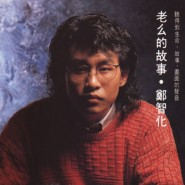
\includegraphics[scale = 0.80]{z/laoyao}
% 	  \caption[labelInTOC]{老妖的故事}
	  \label{fig:laoyao}
	\end{center}
\end{figure}

\begin{songs}{}
  \beginsong{老幺的故事}[index={老幺的故事}]
	黑色的煤渣 \hspace{5 mm} 白色的雾	\\
	阿爸在坑里不断的挖	\\
	养活我们这一家	\\
	骄纵的老幺 \hspace{5 mm} 倔强的我	\\
	命运是什么我不懂	\\
	都市才有我的梦	\\
	\vspace{2ex}
	纠缠的房屋 单纯的心	\\
	坑里的宝藏不再有	\\
	为何我们不搬走	\\
	沉淀的悸动 醉人的酒	\\
	阿爸的嘴角喃喃地说	\\
	这里才有老朋友	\\
	\vspace{2ex}
	通往坑口的那一条路	\\
	不是人生的唯一的方向	\\
	晨曦中模糊的脚步声	\\
	已忘了最后的一次道别	\\
	谁说宠坏的孩子不哭	\\
	就在悲剧发生的那一瞬间	\\
	泪水吶喊唤不回	\\
	阿爸在淹没的矿坑里面	\\
	\vspace{2ex}
	淹没的矿坑它淹没了我的梦	\\
	淹没的矿坑淹没多少笑容	\\
	焚烧的纸钱在狂风中乱飞	\\
	过去的回忆 抹不去的伤痕	\\
	矿工的儿子 逃离家乡的老幺	\\	
	万能的神啊 教我该如何祷告	\\	
	\vspace{2ex}	
	在物质文明的现代战场	\\
	我得到了一切却失去了自己	\\
	再多的梦也填不满空虚	\\
	真情像煤渣化成了灰烬	\\
	家乡的人被矿坑淹没失去了生命	\\
	都市的人被欲望淹没却失去了灵魂	\\
	淹没的矿坑它淹没了我的梦	\\
	淹没的矿坑淹没多少笑容	\\
	淳朴的脸孔又再一次想起	\\
	心灵的归宿何处挡风遮雨	\\
	成长的老幺现在我终于知道	\\
	逃离的家乡最后归去的地方	\\
  \endsong
\end{songs}
